\section{Einleitung}

%\begin{frame}
%	 \frametitle{Übersicht}
%	 \tableofcontents[currentsection]
% \end{frame}

\subsection{Was ist LaTeX?}

\begin{frame}
	\begin{block}{LaTeX}
		\begin{itemize}[<+->]
			\item \textbf{LaTeX} ist ein Textsatzprogramm für \textbf{TeX}
			\item Kein \textbf{WYSIWYG} System wie Microsoft Office / Open Office
			\item Ausgereifter Formelsatz mit vielen Möglichkeiten
			\item Unzählige Erweiterungen
		\end{itemize}
	\end{block}
\end{frame}

\begin{frame}
	\begin{block}{LaTeX - Anwendungen}
		\begin{itemize}[<+->]
			\item Arbeiten (Hausarbeiten, Seminararbeiten, Diplomarbeiten, etc)
			\item Präsentationen
			\item Ausgabe als PDF oder Postscript
		\end{itemize}
	\end{block}
\end{frame}

\subsection{Übersetzung}

\begin{frame}
	\begin{block}{LaTeX}
  \begin{figure}
    \centering
    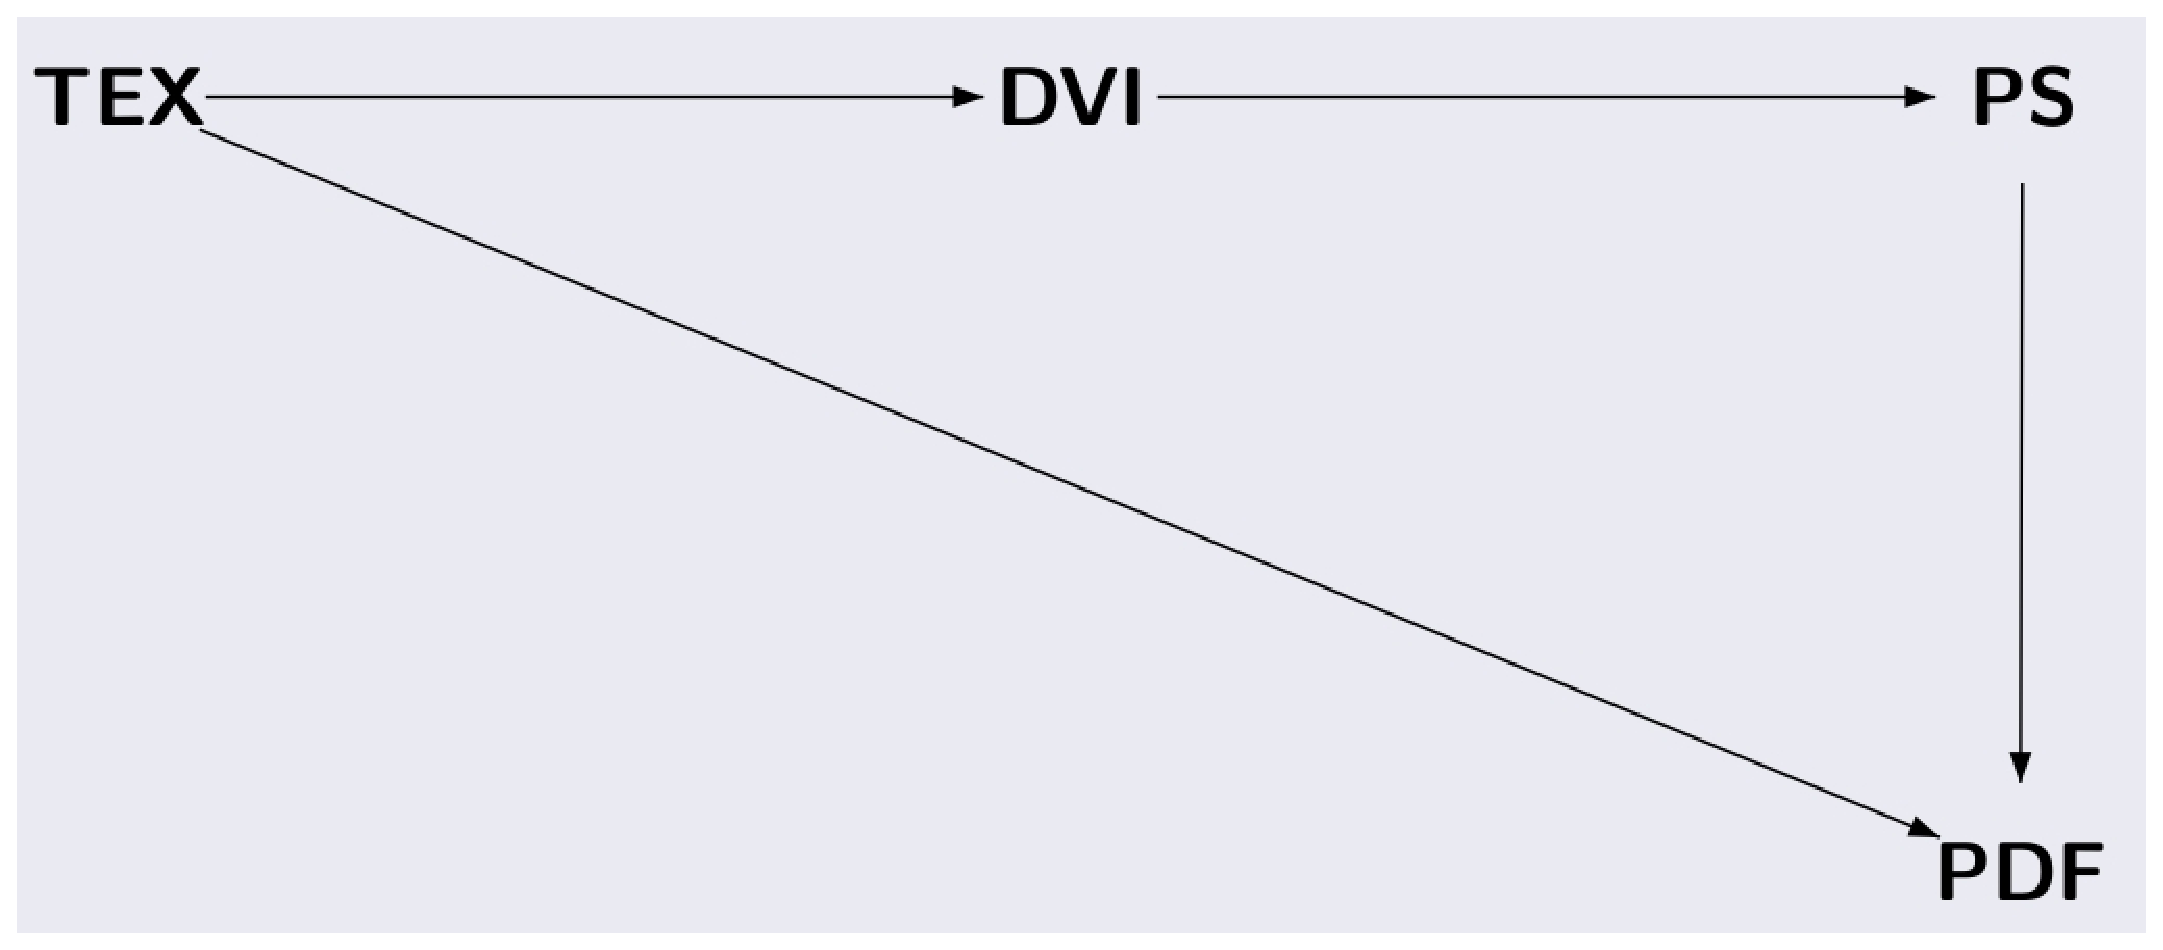
\includegraphics[width=0.8\textwidth]{images/Auswahl_049.eps}
  \end{figure}
	\end{block}
\end{frame}

\begin{frame}[fragile]
	\frametitle{Übersetzung}
	\begin{block}{Quelltext kompilieren}
		\begin{verbatim}
			latex TeXDatei.tex
			pdflatex TeXDatei.tex
		\end{verbatim}
	\end{block}
\end{frame}

\begin{frame}[fragile]
	\frametitle{Übersetzung mit latex}
	\begin{block}{Quelltext kompilieren}
		\begin{verbatim}
			latex TeXDatei.tex

			dvips TeXDatei.dvi

			ps2pdf TeXDatei.ps
		\end{verbatim}
	\end{block}
\end{frame}

\begin{frame}[fragile]
	\frametitle{Übersetzung mit pdflatex}

	Da es für den Anfang komplett ausreichend ist werden wir pdflatex verwenden.
	\pause
	\begin{block}{Quelltext kompilieren}
		\begin{verbatim}
			pdflatex TeXDatei.tex
		\end{verbatim}
	\end{block}
	\pause
	\begin{alertblock}{Achtung}
		Für Fortgeschrittene: Einfach einzubinden kann aber keinen \textit{gastex} Code interpretieren!
	\end{alertblock}
\end{frame}




% Editoren
\subsection{Editoren}

\begin{frame}
	\frametitle{Eine kleine Auswahl}
	\begin{block}{Windows}
		\begin{itemize}
			\item TeXstudio
			\item TEXnicCenter
		\end{itemize}
	\end{block}
	\pause
	\begin{block}{Linux}
		\begin{itemize}
			\item TeXstudio
			\item TEXMaker
			\item Konsole
		\end{itemize}
	\end{block}
	\pause
	\begin{block}{Mac}
		\begin{itemize}
			\item Wie unter Linux
		\end{itemize}
	\end{block}
\end{frame}
